% ------------------------------------------------------------------------------
% TYPO3 CMS 6.2 LTS - What's New - Chapter "In-Depth Changes" (English Version)
%
% @author	Michael Schams <schams.net>
% @license	Creative Commons BY-NC-SA 3.0
% @link		http://typo3.org/download/release-notes/whats-new/
% @language	English
% ------------------------------------------------------------------------------
% Chapter: In-Depth Changes
% ------------------------------------------------------------------------------

\section{In-Depth Changes}
\begin{frame}[fragile]
	\frametitle{In-Depth Changes}

	\begin{center}\huge{Chapter 6:}\end{center}
	\begin{center}\huge{\color{typo3darkgrey}\textbf{In-Depth Changes}}\end{center}

\end{frame}

% ------------------------------------------------------------------------------
% normalize.css
% ------------------------------------------------------------------------------
% http://forge.typo3.org/issues/47920

\begin{frame}[fragile]
	\frametitle{In-Depth Changes}
	\framesubtitle{Normalize.css}

	\begin{itemize}
		\item Backend user interface makes use of \texttt{normalize.css},\newline
			which makes browsers render all elements more consistently and in line with modern standards
		\item Modern, HTML5-ready, alternative to the traditional CSS reset
		\item Aims of \texttt{normalize.css} are:

			\begin{itemize}
				\item Preserve useful browser defaults rather than erasing them
				\item Normalize styles for a wide range of HTML elements
				\item Correct bugs and common browser inconsistencies
				\item Improve usability with subtle improvements
				\item Explain the code using comments and detailed documentation
			\end{itemize}

	\end{itemize}

\end{frame}

% ------------------------------------------------------------------------------
% displayCond options BIT and !BIT
% ------------------------------------------------------------------------------
% http://forge.typo3.org/issues/45514

\begin{frame}[fragile]
	\frametitle{In-Depth Changes}
	\framesubtitle{TCA: displayCond Options BIT And !BIT}

	\lstset{
		basicstyle=\tiny\ttfamily
	}

	\begin{itemize}
		\item Check with a multi-value field in \texttt{displayCond} (bitwise)\newline
			\texttt{BIT}: bit is set, \texttt{!BIT}: bit is \underline{not} set
	\end{itemize}

	\begin{columns}[T]

		\begin{column}{.5\textwidth}

			\advance\leftskip+1cm
			Assuming this TCA:

			\lstset{xleftmargin=1cm}

			\begin{lstlisting}
				'content' => array(
				  'label' => '...',
				  'config' => array(
				    'type' => 'check',
				    'items' => array(
				      array('Content A', ''),
				      array('Content B', ''),
				      array('Content C', ''),
				    ),
				  )
				),
			\end{lstlisting}

		\end{column}
		\begin{column}{.5\textwidth}

			Examples:

			\begin{lstlisting}
				'content_a' => array(
				  'label' => '...',
				  'displayCond' => 'FIELD:content:BIT:1',
				  'config' => array(
				    'type' => 'text',
				  )
				),

				'content_b' => array(
				  'label' => '...',
				  'displayCond' => 'FIELD:content:!BIT:2',
				  'config' => array(
				    'type' => 'text',
				  )
				),
			\end{lstlisting}
		\end{column}

	\end{columns}

\end{frame}

% ------------------------------------------------------------------------------
% Automatic language updates for extensions
% ------------------------------------------------------------------------------
% http://forge.typo3.org/issues/43703

\begin{frame}[fragile]
	\frametitle{In-Depth Changes}
	\framesubtitle{Language Updates}

	\begin{itemize}
		% \item Extbase Command Controller allows to update translations of extensions for selected languages
		\item Extbase Command Controller allows language updates for extensions:

			\begin{lstlisting}
				$GLOBALS['TYPO3_CONF_VARS']['SC_OPTIONS']['extbase']
				  ['commandControllers'][] =
				  'TYPO3\\CMS\\Lang\\Command\\LanguageCommandController';
			\end{lstlisting}

		\item Example call:

			\lstinline!typo3/cli_dispatch.phpsh extbase language:update de,en,fr!

		\item Comma-separated list of locales (e.g. \texttt{de,en,fr}) limits the update to these languages
		\item Without this argument, all languages which are set in module "Languages" are updated

	\end{itemize}

\end{frame}

% ------------------------------------------------------------------------------
% Migrate system extension manuals to reStructuredText
% ------------------------------------------------------------------------------
% http://forge.typo3.org/issues/50052

\begin{frame}[fragile]
	\frametitle{In-Depth Changes}
	\framesubtitle{System Extensions: ReST Manuals}

	\begin{itemize}
		\item All system extension manuals are migrated to reStructuredText
		\item OpenOffice manuals are not longer used and have been removed
		\item ReST is an easy-to-read, what-you-see-is-what-you-get plaintext markup syntax and parser system
		\item ReST files of system extensions are stored in:\newline
			\texttt{typo3/sysext/<extensionkey>/Documentation/*}

		\item Further information:

			\begin{itemize}
				\item \url{http://de.wikipedia.org/wiki/ReStructuredText}
				\item \url{http://wiki.typo3.org/ReST}
			\end{itemize}

	\end{itemize}

\end{frame}

% ------------------------------------------------------------------------------
% Support custom translation servers for extensions
% ------------------------------------------------------------------------------
% http://forge.typo3.org/issues/50052

\begin{frame}[fragile]
	\frametitle{In-Depth Changes}
	\framesubtitle{Custom Translation Servers}

	\begin{itemize}
		\item Support of custom translation servers for extensions was implemented
		\item With the use of XLIFF and a new Signal/Slot,\newline
			this becomes a no-brainer (see next slide for an example)
		\item A possible translation server solution: \textbf{Pootle}

			\begin{itemize}
				\item online translation management tool with translation interface
				\item written in the Python/Django
				\item originally developed and released by \url{translate.org.za}
				\item GNU GPL license
			\end{itemize}

	\end{itemize}

\end{frame}

% ------------------------------------------------------------------------------
% Support custom translation servers for extensions
% ------------------------------------------------------------------------------
% http://forge.typo3.org/issues/50052

\begin{frame}[fragile]
	\frametitle{In-Depth Changes}
	\framesubtitle{Custom Translation Servers}

	Example: \texttt{EXT:myextension/localconf.php}

	\lstset{
		basicstyle=\tiny\ttfamily
	}

	\begin{lstlisting}
		/**
		 * @var \TYPO3\CMS\Extbase\SignalSlot\Dispatcher $signalSlotDispatcher
		 */
		$signalSlotDispatcher =
		  \TYPO3\CMS\Core\Utility\GeneralUtility::makeInstance(
		    'TYPO3\\CMS\\Extbase\\SignalSlot\\Dispatcher');

		$signalSlotDispatcher->connect(
		  'TYPO3\\CMS\\Lang\\Service\\UpdateTranslationService',
		  'postProcessMirrorUrl',
		  'Company\\Extension\Slots\\CustomMirror',
		  'postProcessMirrorUrl'
		);
	\end{lstlisting}

\end{frame}

% ------------------------------------------------------------------------------
% Support custom translation servers for extensions
% ------------------------------------------------------------------------------
% http://forge.typo3.org/issues/50052

\begin{frame}[fragile]
	\frametitle{In-Depth Changes}
	\framesubtitle{Custom Translation Servers}

	Example: \texttt{EXT:myextension/Classes/Slots/CustomMirror.php}

	\lstset{
		basicstyle=\tiny\ttfamily
	}

	\begin{lstlisting}
		<?php
		namespace Company\Extensions\Slots;
		class CustomMirror {

		  /**
		   * @var string
		   */
		  protected static $extKey = 'myextension';

		  public function postProcessMirrorUrl($extensionKey, &$mirrorUrl) {
		    if ($extensionKey === self::$extKey) {
		      $mirrorUrl = 'http://example.com/typo3-packages/';
		    }
		  }

		}
	\end{lstlisting}

\end{frame}

% ------------------------------------------------------------------------------
% Support custom translation servers for extensions
% ------------------------------------------------------------------------------
% http://forge.typo3.org/issues/50052

\begin{frame}[fragile]
	\frametitle{In-Depth Changes}
	\framesubtitle{Custom Translation Servers}

	Expected file/directory structure on server:

	\begin{lstlisting}
		http://example.com/typo3-packages/
		 `-- <first-letter-of-extension-key>
		     `-- <second-letter-of-extension-key>
		         `-- <extension-key>-l10n
		             |-- <extension-key>-l10n-de.zip
		             |-- <extension-key>-l10n-fr.zip
		             |-- <extension-key>-l10n-it.zip
		             `-- <extension-key>-l10n.xml
	\end{lstlisting}

	For example:

	\begin{lstlisting}
		http://example.com/typo3-packages/m/y/myextension-l10n/myextension-l10n.xml
	\end{lstlisting}

\end{frame}

% ------------------------------------------------------------------------------
% Support custom translation servers for extensions
% ------------------------------------------------------------------------------
% http://forge.typo3.org/issues/50052

\begin{frame}[fragile]
	\frametitle{In-Depth Changes}
	\framesubtitle{Custom Translation Servers}

	Example: \texttt{<extension-key>-l10n.xml}

	\lstset{
		basicstyle=\tiny\ttfamily
	}

	\begin{lstlisting}
		<?xml version="1.0" standalone="yes" ?>
		  <TERlanguagePackIndex>
		    <meta>
		      <timestamp>1374841386</timestamp>
		      <date>2013-07-26 14:23:06</date>
		    </meta>
		    <languagePackIndex>
		    <languagepack language="de">
		      <md5>1cc7046c3b624ba1fb1ef565343b84a1</md5>
		    </languagepack>
		    <languagepack language="fr">
		     <md5>f00f73ae5c43cb68392e6c508b65de7a</md5>
		    </languagepack>
		    <languagepack language="it">
		     <md5>cd59530ce1ee0a38e6309544be6bcb3d</md5>
		    </languagepack>
		  </languagePackIndex>
		</TERlanguagePackIndex>
	\end{lstlisting}

\end{frame}

% ------------------------------------------------------------------------------
% Automatic import of t3d files for extensions
% ------------------------------------------------------------------------------
% http://forge.typo3.org/issues/51437

\begin{frame}[fragile]
	\frametitle{In-Depth Changes}
	\framesubtitle{Automatic t3d Import}

	\begin{itemize}
		\item Extensions can now import initial \textbf{t3d packages} automatically\newline
			upon extension installation
		\item t3d files contain things such as data, relations, files, etc.
		\item The t3d file has to be named \texttt{data.t3d} and located in:\newline
			\texttt{EXT:myextension/Initialisation/}

		\item Import happens \underline{once} only\newline
			(even if the extension is re-installed later)

	\end{itemize}

\end{frame}

% ------------------------------------------------------------------------------
% Automatic import of files for extensions
% ------------------------------------------------------------------------------
% http://forge.typo3.org/issues/51446

\begin{frame}[fragile]
	\frametitle{In-Depth Changes}
	\framesubtitle{Automatic File Import}

	\begin{itemize}
		\item Extensions can now import initial \textbf{files} automatically\newline
			upon extension installation
		\item Files have to be located in:\newline
			\texttt{EXT:myextension/Initialisation/Files/...}
		\item Files are copied to:\newline
			\texttt{fileadmin/<extensionkey>/}
		\item Import happens \underline{once} only\newline
			(even if the extension is re-installed later)

	\end{itemize}

\end{frame}

% ------------------------------------------------------------------------------
% Use an extension as repository
% ------------------------------------------------------------------------------
% http://forge.typo3.org/issues/51835

\begin{frame}[fragile]
	\frametitle{In-Depth Changes}
	\framesubtitle{Use An Extension As Repository}

	\begin{itemize}
		\item Sometimes extensions depend on customized versions of other extensions or on extensions which have not been released to the official TYPO3 Extension Repository (TER)
		\item To address this issue, extensions can now be shipped with "other" extensions
		\item These have to be located in (unpacked):\newline
			\texttt{EXT:myextension/Initialisation/Extensions/...}

		\item Upon extension installation, they are copied to:\newline
			\texttt{typo3conf/ext/}

		\item After that, extension dependencies are resolved

	\end{itemize}

\end{frame}

% ------------------------------------------------------------------------------
% CLI command to install/uninstall extensions
% ------------------------------------------------------------------------------
% http://forge.typo3.org/issues/51629

\begin{frame}[fragile]
	\frametitle{In-Depth Changes}
	\framesubtitle{Install/uninstall extensions via CLI}

	\begin{itemize}
		\item Install and uninstall extensions by command line interface (CLI)
		\item Examples:
			\lstinline!typo3/cli_dispatch.phpsh extbase extension:install <extensionkey>!
			\lstinline!typo3/cli_dispatch.phpsh extbase extension:uninstall <extensionkey>!

		\item Note: a backend user \textbf{\_cli\_lowlevel} is required for that
	\end{itemize}

\end{frame}

% ------------------------------------------------------------------------------
% Enable/disable cascading deletion of child elements
% ------------------------------------------------------------------------------
% http://forge.typo3.org/issues/50391

\begin{frame}[fragile]
	\frametitle{In-Depth Changes}
	\framesubtitle{Cascading Deletion Of Child Elements}

	\begin{itemize}
		\item TCA now features a setting to enable/disable cascading deletion of child elements
		\item Relation must be of type "\textbf{inline}"
		\item Default value is \texttt{TRUE} (deletion of inline child records is enabled)
		\item Example (disable deletion of inline child records):

			\begin{lstlisting}
				...
				'type' => 'inline',
				'foreign_table' => ...,
				  'behaviour' => array(
				    'enableCascadingDelete' => 0
				  )
				  ...
				)
				...
			\end{lstlisting}

	\end{itemize}

\end{frame}

% ------------------------------------------------------------------------------
% Multiple category fields per table
% ------------------------------------------------------------------------------
% http://forge.typo3.org/issues/51921

\begin{frame}[fragile]
	\frametitle{In-Depth Changes}
	\framesubtitle{Multiple Category Fields Per Table}

	\begin{itemize}
		\item In TYPO3 < 6.2, it is only possible to do \underline{one} \texttt{makeCategorizable()} call per table
			(multiple calls would overwrite previous category field declarations)
		\item Since TYPO3 >= 6.2, multiple category fields per table are possible
		\item Example:

			\begin{lstlisting}
				\TYPO3\CMS\Core\Utility\ExtensionManagementUtility::makeCategorizable(
				  $extensionKey,
				  $tableName,
				  $fieldName = 'categories',
				  $options = array(
				  	'label' => 'my category'
				  )
				);
			\end{lstlisting}

		\item Custom labels for each category field can be set in array \texttt{\$options}

	\end{itemize}

\end{frame}

% ------------------------------------------------------------------------------
% Backend layout data providers
% ------------------------------------------------------------------------------
% http://forge.typo3.org/issues/37208

\begin{frame}[fragile]
	\frametitle{In-Depth Changes}
	\framesubtitle{Backend Layout Data Providers}

	\begin{itemize}
		\item In TYPO3 < 6.2, backend layouts are stored in the DB as regular records
		\item Since TYPO3 >= 6.2, so-called \emph{data providers} can be defined\newline
			\small(for example to enable extensions to ship their own backend layout definitions from static files)\normalsize

		\item Data providers have to implement the interface:\newline
			\smaller\texttt{
				TYPO3\textbackslash\textbackslash
				CMS\textbackslash\textbackslash
				Backend\textbackslash\textbackslash
				View\textbackslash\textbackslash
				BackendLayout\textbackslash\textbackslash
				DataProviderInterface}\normalsize

		\item and can be registered by:

			\begin{lstlisting}
				$GLOBALS['TYPO3_CONF_VARS']['SC_OPTIONS']
				  ['BackendLayoutDataProvider'][$_EXTKEY] = 'Classname';
			\end{lstlisting}


	\end{itemize}

\end{frame}

% ------------------------------------------------------------------------------
% Backend layout data providers
% ------------------------------------------------------------------------------
% http://forge.typo3.org/issues/37208

\begin{frame}[fragile]
	\frametitle{In-Depth Changes}
	\framesubtitle{Backend Layout Data Providers}

	\begin{itemize}
		\item New API functions for handling of backend layout data providers:

			\begin{lstlisting}
				'itemsProcFunc' => 'TYPO3\\CMS\\Backend\\View\\
				  BackendLayoutView->addBackendLayoutItems'
			\end{lstlisting}

			\begin{lstlisting}
				getBackendLayoutView()->getSelectedCombinedIdentifier($id);
				getBackendLayoutView()->getSelectedBackendLayout();
			\end{lstlisting}

		\item New PageTSconfig option to exclude backend layouts:

			\begin{lstlisting}
				options.backendLayout.exclude = default_1, my_extension__headerLayout
			\end{lstlisting}

	\end{itemize}

\end{frame}

% ------------------------------------------------------------------------------
% Filter for multiple value selector
% ------------------------------------------------------------------------------
% http://forge.typo3.org/issues/49739

\begin{frame}[fragile]
	\frametitle{In-Depth Changes}
	\framesubtitle{Multiple Value Selector (1)}

	\lstset{
		basicstyle=\tiny\ttfamily
	}

	\begin{itemize}
		\item Filter available items in a multi-select element (by TCA settings)
		\item For example: enable a text field for individual word filter and pre-define search words a user can select from a drop down box

		\item To use this new feature, adjust TCA accordingly\newline
			(e.g. in file \texttt{typo3conf/extTables.php}):


			\begin{lstlisting}
				$GLOBALS['TCA']['fe_users']['columns']['usergroup']['config']
				  ['enableMultiSelectFilterTextfield'] = TRUE;

				$GLOBALS['TCA']['fe_users']['columns']['usergroup']['config']
				  ['multiSelectFilterItems'] = array(

				  array('',     'show all'),  // no filter
				  array('test', 'test'),      // first value: filter, second value: label

				  array(
				    'TYPO3',
				    'LLL:EXT:myext/Resources/Private/Language/locallang_db.xlf:tx_myext.label.typo3'
				  ),
				);
			\end{lstlisting}

	\end{itemize}

\end{frame}

% ------------------------------------------------------------------------------
% Filter for multiple value selector
% ------------------------------------------------------------------------------
% http://forge.typo3.org/issues/49739

\begin{frame}[fragile]
	\frametitle{In-Depth Changes}
	\framesubtitle{Multiple Value Selector (2)}

	\begin{itemize}
		\item Two options are available:

			\begin{itemize}
				\item Select pre-defined values from dropdown box
				\item Enter search/filter keyword in an input field
			\end{itemize}

		\item The result could look like:
	\end{itemize}

	\begin{figure}
		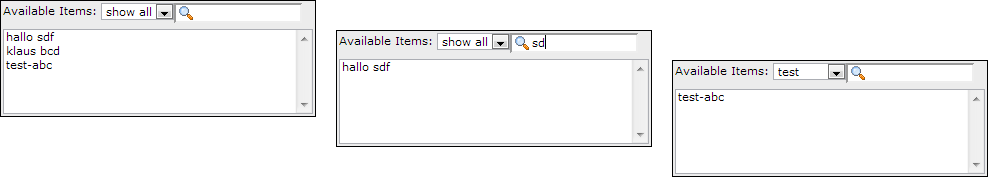
\includegraphics[width=1\linewidth]{Images/InDepthChanges/MultipleValueSelector.png}
	\end{figure}

\end{frame}

% ------------------------------------------------------------------------------
% Improved caching framework by introducing cache groups
% (slide added in March 2014)
% ------------------------------------------------------------------------------
% http://forge.typo3.org/issues/54991

\begin{frame}[fragile]
	\frametitle{In-Depth Changes}
	\framesubtitle{Cache Groups (1)}

	\begin{itemize}
		\item TYPO3 core uses two types of caches:

			\begin{itemize}
				\item \textbf{system-related caches}:
				class loading cache, configuration cache, l10n\_cache, extbase\_object, extbase\_reflection etc.
				\item \textbf{frontend-related caches}:
				cHash cache, page cache, page section cache
			\end{itemize}

		\item In TYPO3 < 6.2, \textit{clear all caches} empties \underline{all} caches, which is not ideal

		\item In TYPO3 >= 6.2, the core uses two cache groups:\newline
			"\textbf{pages}" with all page-related caches and "\textbf{system}", which is used for compile-time and configuration caches

	\end{itemize}

	\begin{figure}
		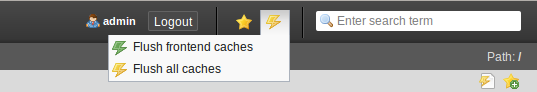
\includegraphics[width=0.5\linewidth]{Images/InDepthChanges/CacheGroups.png}
	\end{figure}

\end{frame}

% ------------------------------------------------------------------------------
% Improved caching framework by introducing cache groups
% (slide added in March 2014)
% ------------------------------------------------------------------------------
% http://forge.typo3.org/issues/54991

\begin{frame}[fragile]
	\frametitle{In-Depth Changes}
	\framesubtitle{Cache Groups (2)}

	\lstset{
		basicstyle=\tiny\ttfamily
	}

	\begin{itemize}

		\item Relevant configuration option:\newline
			\smaller(in files: \texttt{LocalConfiguration.php}/\texttt{DefaultConfiguration.php})\normalsize

			\begin{lstlisting}
			'cache_hash' => array(
			  'frontend' => 'TYPO3\CMS\Core\Cache\Frontend\VariableFrontend',
			  'backend' => 'TYPO3\CMS\Core\Cache\Backend\Typo3DatabaseBackend',
			  'options' => array(),
			  'groups' => array('pages', 'all')
			),
			\end{lstlisting}

		\item "\textit{Flush all caches}" command does not flush system-related caches any more
			(only "Clear Configuration Cache" or the Install Tool empty these caches)
		\item A new userTSconfig option enables non-admins to clear system caches:\newline
			\smaller\texttt{options.clearCache.system = 1}\normalsize

		\breakingchange

	\end{itemize}

\end{frame}

% ------------------------------------------------------------------------------
% TCA: limit number of ticked checkboxes
% (slide added in March 2014)
% ------------------------------------------------------------------------------
% http://forge.typo3.org/issues/55187
% http://forge.typo3.org/issues/55188 (documentation: TCA reference)

\begin{frame}[fragile]
	\frametitle{In-Depth Changes}
	\framesubtitle{TCA: Number of Ticked Checkboxes}

	\lstset{
		basicstyle=\tiny\ttfamily
	}

	\begin{itemize}
		\item TCA allows validation of number of ticked checkboxes

			\begin{itemize}
				\item \texttt{maximumRecordsChecked}:\newline
					limit number of records system-wide
				\item \texttt{maximumRecordsCheckedInPid}:\newline
					limit number of records PID-wide (parent ID)
			\end{itemize}

		\item If a BE user exceeds the max number, the additional tick gets reverted until another record is unchecked

		\item Example:

			\begin{lstlisting}
				$tcaConfiguration = array(
				  'type' => 'check',
				  'eval' => 'maximumRecordsChecked',
				  'validation' => array(
				    'maximumRecordsChecked' => 5
				  )
				);
			\end{lstlisting}

	\end{itemize}

\end{frame}

% ------------------------------------------------------------------------------
% TCA: Introduce MM_oppositeUsage property
% (slide added in March 2014)
% ------------------------------------------------------------------------------
% http://forge.typo3.org/issues/56061
% http://forge.typo3.org/issues/56123 (documentation: TCA reference)

\begin{frame}[fragile]
	\frametitle{In-Depth Changes}
	\framesubtitle{TCA: \texttt{MM\_oppositeUsage} property}

	\lstset{
		basicstyle=\tiny\ttfamily
	}

	\begin{itemize}
		\item On copying a \texttt{sys\_category} record, a new MM reference is created, but without setting the "fieldname"
		\item This value is basically defined from the opposite entity with \texttt{MM\_match\_fields}, but cannot be accessed
		\item To address this issue, a new property \texttt{MM\_oppositeUsage} has been introduced for the TCA:

			\begin{lstlisting}
				'config' => array(
				  'allowed' => '*',
				  'MM' => 'tx_myextension_first_second_mm',
				  'MM_oppositeUsage' => array(
				    'tt_content' => array('somefield'),
				    'tx_myextension_domain_model' => array('some_property'),
				  ),
				),
			\end{lstlisting}

	\end{itemize}

\end{frame}

% ------------------------------------------------------------------------------
% Miscellaneous
% ------------------------------------------------------------------------------
% http://forge.typo3.org/issues/49037 (Custom record list in element browser)
% http://forge.typo3.org/issues/36505 (Increase size of be_groups.subgroup field)
% http://forge.typo3.org/issues/49270 (Merge extensions TS/Template)

\begin{frame}[fragile]
	\frametitle{In-Depth Changes}
	\framesubtitle{Miscellaneous}

	\begin{itemize}

		\item \textbf{Custom record list:}\newline
			\small
				A custom record list instance can be used in the element browser to override the default element browser record list
			\normalsize

		\item \textbf{More subgroups:}\newline
			\small
				Attribute \texttt{subgroup} in DB table \texttt{be\_groups} changed from \texttt{varchar(250)} to \texttt{text}, which allows for much more subgroups (backend users/groups)
			\normalsize

		\item \textbf{Extensions TS/Template merged:}\newline
			\small
				Technically, "WEB > Template" was spread among several extensions (tstemplate\_ceditor, tstemplate\_info, tstemplate\_objbrowser and tstemplate\_analyzer). Those extensions are now merged into one single extension: "tstemplate"
			\normalsize

	\end{itemize}
	
\end{frame}

% ------------------------------------------------------------------------------
% Miscellaneous
% ------------------------------------------------------------------------------
% http://forge.typo3.org/issues/49721 (Add label_userFunc_options support to BackendUtility)
% http://forge.typo3.org/issues/50441 (Add a timestamp when downloading an extension)
% http://forge.typo3.org/issues/51352 (Force saltedpasswords for Backend)

\begin{frame}[fragile]
	\frametitle{In-Depth Changes}
	\framesubtitle{Miscellaneous}

	\begin{itemize}

		\item \textbf{label\_userFunc\_options:}\newline
			\small
				Support of \texttt{label\_userFunc\_options} added to \texttt{BackendUtility}
			\normalsize

		\item \textbf{Extension filename:}\newline
			\small
				When downloading an extension in the Extension Manager, filename contains timestamp (year, month, day and time):\newline
				\texttt{<extensionKey>\_<version>\_<timestamp>.zip}\newline
				\texttt{myextension\_1.0.0\_201312102359.zip}
			\normalsize

		\item \textbf{EXT:saltedpasswords:}\newline
			\small
				Extension EXT:saltedpasswords is a required system extension and enabled by default now.
				This forces salted hashes for backend authentication. The Install Tool checks settings and adapts them if required.
			\normalsize

	\end{itemize}
	
\end{frame}

% ------------------------------------------------------------------------------
% Miscellaneous
% ------------------------------------------------------------------------------
% http://forge.typo3.org/issues/51138 (Allow SignalSlots to modify arguments)
% http://forge.typo3.org/issues/31996 (Transfer query parameters in preview)
% http://forge.typo3.org/issues/52630 (TCEforms PlaceHolder works recursively now)

\begin{frame}[fragile]
	\frametitle{In-Depth Changes}
	\framesubtitle{Miscellaneous}

	\begin{itemize}

		\item \textbf{SignalSlots to modify arguments:}\newline
			\small
				Arguments passed to SignalSlots dispatcher can be modified now and dispatcher returns the (modified) arguments as it received them in order to keep chaining intact.
			\normalsize

		\item \textbf{Workspace preview:}\newline
			\small
				Query parameters are passed to workspace preview now. This was a problem in TYPO3 < 6.2, where extensions passing custom parameters do not work properly.
			\normalsize

		\item \textbf{TCEforms PlaceHolder feature:}\newline
			\small
				Introduced in TYPO3 CMS 4.7, the PlaceHolder features of TCEforms works recursively now (e.g. \texttt{\_\_row|uid\_foreign|field}).
			\normalsize

	\end{itemize}
	
\end{frame}

% ------------------------------------------------------------------------------
% Miscellaneous
% ------------------------------------------------------------------------------
% http://forge.typo3.org/issues/14730 (Support for proxy NTLM authentication)
% http://forge.typo3.org/issues/49667 (Enable double-resolution icons in SpriteGenerator)

\begin{frame}[fragile]
	\frametitle{In-Depth Changes}
	\framesubtitle{Miscellaneous}

	\begin{itemize}

		\item \textbf{Double-resolution icons:}\newline
			\small
				SpriteManager supports high resolution icons now: it generates a second sprite with double sized icons (a second file with "@x2.png" suffix). CSS3 ensures, that the high-res file is loaded on devices which support this\newline
				(this does not affect performance on other devices).
			\normalsize

		\item \textbf{Proxy NTLM authentication:}\newline
			\small
				Support for proxy NTLM authentication (\textbf{NT} \textbf{L}AN \textbf{M}anager: a suite of Microsoft security protocols) added. This feature can be activated in the Install Tool:\newline
			\normalsize
			\smaller
				\texttt{\$GLOBALS['TYPO3\_CONF\_VARS']['SYS']['curlProxyNTLM']}\newline
				\emph{(by the way: this feature was requested more than 8 years ago :-)}
			\normalsize

	\end{itemize}
	
\end{frame}

% ------------------------------------------------------------------------------
% Miscellaneous
% (slide added in March 2014)
% ------------------------------------------------------------------------------
% http://forge.typo3.org/issues/14730 (Support for proxy NTLM authentication)

\begin{frame}[fragile]
	\frametitle{In-Depth Changes}
	\framesubtitle{Miscellaneous}

	\begin{itemize}

		\item \textbf{cookieHttpOnly by default:}\newline
			\small
				In order to make the session cookie only accessible through the HTTP protocol, \texttt{cookieHttpOnly} is enabled by default now.\newline
				This means, cookies "fe\_typo\_user" and "be\_typo\_user" will not be accessible by scripting languages (e.g. JavaScript), which hardens the protection against XSS attacks (\textit{cross site scripting}). Although, some older browsers do not support this technique.
			\normalsize

		\item \textbf{Clean-up Database Table:}\newline
			\small
				Following attributes removed from DB table \texttt{tt\_content} (not used since TYPO3 4.0):
				\texttt{text\_align}, \texttt{text\_face}, \texttt{text\_size}, \texttt{text\_color}, \texttt{text\_properties}.
			\normalsize

	\end{itemize}
	
\end{frame}

% ------------------------------------------------------------------------------
% Miscellaneous
% (slide added in March 2014)
% ------------------------------------------------------------------------------
% https://forge.typo3.org/issues/55190 (Move Tidy functionality to a TER extension)

\begin{frame}[fragile]
	\frametitle{In-Depth Changes}
	\framesubtitle{Miscellaneous}

	\begin{itemize}

		\item \textbf{HTML Tidy removed:}\newline
			\small
				The \textit{HTML Tidy} functionality has been removed from the TYPO3 core. It can easily be re-instituted by installing EXT:tidy from the TER.
			\normalsize

		\item \textbf{dontSetCookie removed:}\newline
			\small
				Due to the fact that the cookie "fe\_typo\_user" is only set if required (and not always), the Install Tool option \texttt{dontSetCookie} became irrelevant and has been removed.
			\normalsize

		\item \textbf{"Wizard" scripts removed:}\newline
			\small
				Removal of the following "wizard" scripts:
				\texttt{typo3/wizard\_add.php}, \texttt{typo3/wizard\_colorpicker.php}, \texttt{typo3/wizard\_edit.php}, \texttt{typo3/wizard\_forms.php}, \texttt{typo3/wizard\_list.php}, \texttt{typo3/wizard\_rte.php}, \texttt{typo3/wizard\_table.php}
			\normalsize

	\end{itemize}
	
\end{frame}

% ------------------------------------------------------------------------------

